\section{Technical Tools} \label{ch:methods:tech}

\subsection{Striatal Lesion} \label{ch:method:lesion}
\begin{figure}[bth!]
	\begin{center}
		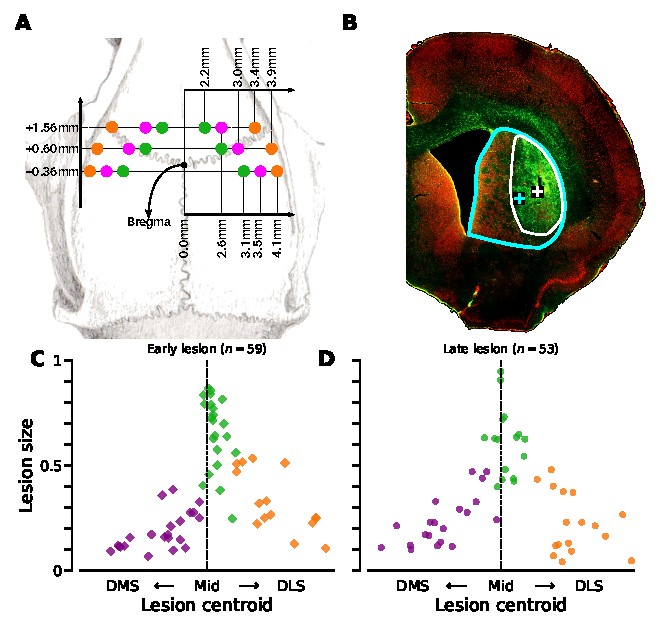
\includegraphics[scale=1]{ch-methods/figures/LesionSizeLocation.pdf}
		\caption
		{\textbf{Dorsal striatum lesion quantification.}
		\textbf{A)} Schematic of the lesion sites.
		\textbf{B)} Illustration of the quantification of the lesion size.
		For each coronal slide and hemi-striatum, the contour of the lesion was manually outlined using the GFAP staining.
		The relative size of the lesion (compared to the full striatum, manually outlined on the NeuN staining) and the coordinates of the lesion/striatum centroid was calculated.
		For each animal, the size and laterality were obtained by averaging data along the anteroposterior axis, for both left and right hemispheres.
		\textbf{C, D)} Lesion size versus laterality for animals that underwent lesion before (Early, \textbf{C}) and after (Late, \textbf{D}) extensive practice.
		Lesion quantification was performed blindly relative to behavioral analysis.
		In four animals with a striatal lesion performed after learning the task (late lesion), the lesion size quantification could not be properly performed.
		These animals were classified according to their injection coordinates in the surgery (3 DLS and 1 DMS), however they were excluded from any analysis that required the lesion size (hence the difference between the number of ``late lesion'' animals in this figure, $n=53$, and the total number of animals in \autoref{fig:lesion:task}, $n=57$).
		}
		\label{fig:method:LesionSizeLocation}
	\end{center}
\end{figure}
Anesthesia was induced with an intraperitoneal (IP) injection of a mixture of 100~mg/kg ketamine and 10~mg/kg xylazine and was maintained during the surgery with inhalant isoflurane gas (less than 3\%).
After shaving and cleaning the scalp, the animal was placed in the stereotaxic frame (Kopf instruments) and a local anesthetic (lidocaine) was injected under the scalp.
Then, an incision along the midline of the skull was made, followed by cleaning the exposed skull and drilling the craniotomies above the targeted areas.
To perform fiber-sparing lesion of the \gls{ds}, ibotenic acid (1\% in 0.1~M~NaOH, Fisher Scientific) was infused (Pump 11 Elite Nanomite, Harvard Apparatus, using a 10~$\mu$L WPI Nanofil syringe) in 6 specular sites bilaterally, at a rate of 90~nL/min.
The needle remained in place for 10~min following the injection to allow for the diffusion of the excitotoxic drug.
Then, the needle was retracted slowly to avoid backflow of the drug.
Once all the injections were performed, craniotomies were filled with bone wax, the skull was disinfected, and the skin was sutured.
Animals were allowed to recover for two weeks before resuming behavioral training.
After surgery, animals were housed alone for 3 days, to avoid getting hurt by the cagemates, and were force-fed if needed.
Injection coordinates (in~mm, with reference to Bregma, according to Paxinos) are shown in \Autoref{fig:method:LesionSizeLocation}{A} (each injection at $-5.6$~mm dorsoventral).
The infused volume in each site was 200~nL for DLS and DMS lesions, and 400~nL for \gls{ds} lesions.

\subsection{Immunohistochemistry}
At the end of the experiments, animals were euthanized with an overdose IP injection of $\sim$2~mL pentobarbital.
Then, they were perfused with 4\% paraformaldehyde and their brains were harvested for histological analysis of the lesion size and location.
Brains were coronally sliced on a vibratome at 60~$\mu$m thickness.
For each animal, six sections spanning the \gls{ds} along the rostrocaudal axis were selected (usually the following slice numbers: 5, 15, 25, 35, 45, and 55 for consistency) and submerged in 0.1~M~PBS.
Then, PBS was replaced with citrate buffer (10~mM) for 10~min at room temperature.
Next, slices were submerged with a blocking solution, consisting of PBS with 0.3\% triton and 15\% normal goat serum (NGS) for 120~min at room temperature.
Then, the solution was replaced with another consisting of 2~$\mu$L anti-NeuN antibody (Merks Millipore, MAB377) and 0.5~$\mu$L of anti-GFAP antibody (Agilent, Z033429-2) diluted in 200~$\mu$L of the blocking solution, kept overnight at 4~\textcelsius.
Sections were then rinsed twice in PBS, 10~min each, at room temperature, before being submerged again in 1~$\mu$L of donkey anti-mouse antibody (Al555, red), 1~$\mu$L of donkey anti-rabbit antibody (Al488, green) diluted in 400~$\mu$L of PBS for 120~min at room temperature.
Finally, they were washed twice in PBS, for 10~min each time, and mounted for microscopy.

\subsection{Lesion Quantification}
Whole slices were imaged using an Apotome microscope (Zeiss, 28126), and stitched together in the processing software (Zeiss Zen).
Then for each slice, the ventricule, the striatum, and the lesioned area were manually outlined (\Autoref{fig:method:LesionSizeLocation}{B}) bilaterally in the image processing software (ImageJ, Fiji).
The size and the centroid coordinates were automatically computed for all of the above-mentioned areas.
Next, the anteroposterior location of each slice was also approximated according to the rat brain atlas (Paxinos).
\par
The lesion size reported in this paper is the ratio of the lesion volume over the volume of the striatum.
Both regions of interest (lesion and striatum) were approximated as a truncated cone between any two consecutive sections, and the volume was accordingly calculated and summed up.
\Autoref{fig:method:LesionSizeLocation}{C-D} show the lesion coordinates of all the animals trained in the normal treadmill task.
The type of the lesion (\gls{dls}, \gls{dms} or \gls{ds}) was determined visually and confirmed by comparing the centroid location of the lesion to that of the entire striatum.
Animals with a \gls{dls} lesion in one hemisphere and a \gls{dms} in another ($n=7$) were excluded from this manuscript.
Four rat brains were imaged improperly, they are automatically removed from any analysis that required the lesion size.


\subsection{Statistics}
All statistical comparisons were performed using resampling methods (permutation test and bootstrapping).
These non-parametric methods alleviate many concerns in traditional statistical hypothesis tests, such as distribution assumptions (e.g., normality assumption under analysis of variance), error inflation due to multiple comparisons, and sensitivity to unbalanced group size.
\par
We used the permutation test to compare the performance of two groups of animals during training on a session-by-session basis, such as in \Autoref{fig:time:varTrd}{b}, and \Autoref{fig:lesion:EarlyLesionLearning}{A}.
To simplify the description~\cite[see][for the complete description]{Fujisawa2008NN}, let's assume, as in \Autoref{fig:time:varTrd}{b}, we have ${\mathbf{X}=[X_1, X_2,...,X_n]}$, where $X_i$ is the set of \glspl{et} of all the animals in session~$i$.
Similarly, we have $\mathbf{Y}$ that contains \glspl{et} from another experimental condition.
Here, the null hypothesis states that the assignment of each data point in $X_i$ and $Y_i$ to either $\mathbf{X}$ or $\mathbf{Y}$ is random, hence there is no difference between $\mathbf{X}$ and $\mathbf{Y}$.
\par
In short, the test statistic was defined as the difference between smoothed (using Gaussian kernel with $\sigma =0.05$) average of $\mathbf{X}$ and $\mathbf{Y}$ for each session~$i$: $D_0(i)$.
I then generated one set of surrogate data by assigning \gls{et} of each animal in session $i$ to either $X_i$ or $Y_i$, randomly.
For each set of surrogate data, the test statistic was similarly calculated, i.e.,~$D_m(i)$.
This process was repeated 10,000 times for all the statistical comparisons in this manuscript, obtaining: $D_1(i),\ldots,D_{10000}(i)$.
\par
At this step, two-tailed pointwise p-values could be directly calculated for each $i$, from the $D_m(i)$ quantiles~\cite{Fujisawa2008NN}.
Moreover, to compensate for the issue of multiple comparisons, we defined global bands of significant differences along the session index dimension.
From 10,000 sets of surrogate data, a band of the largest $\alpha$-percentile was constructed, such that less than 5\% of $D_m(i)$s broke the band at any given session $i$.
This band (denoted as the \textit{global band}) represents the threshold for significance, and any break-point by $D_0(i)$ at any $i$ is a point of significant difference between $\mathbf{X}$ and $\mathbf{Y}$.
\par
A similar permutation test was also used when comparing only two sets of \textit{unpaired} data points (such as in \Autoref{fig:time:shortSharp}{e}, comparing control vs.\ short~GT groups).
The same algorithm was employed, having only one value for index $i$.
If none of the $D_m(i)$s exceeded $D_0(i)$, the value $p<0.0001$ was reported (i.e., less than one chance in 10,000).
\par
For paired comparisons (such as in \Autoref{fig:time:varTrd}{f} and in \Autoref{fig:lesion:rev}{C}), I generated the bootstrap distribution of mean differences ($n=10000$ with replacement).
Significance was reported if 95\% confidence interval (CI) of the pairwise differences differed from zero (i.e., zero was not within the CI)~\cite{Efron1994}.
For example, in \Autoref{fig:time:varTrd}{f, right}, the 95\% CI of pairwise differences is $(19, 27)$.
Since this interval does not contain zero, it is reported significant, whereas in \Autoref{fig:time:shortSharp}{e}, the CI of the comparison between normal and sharp short~GT is $(-0.17, +0.01)$ which includes zero, and hence is reported non-significant.
\par
Exceptionally, for the comparison in \Autoref{fig:time:shortSharp}{h}, even though it is not paired, I used bootstrapping, because I did not have enough data points to perform the permutation test.
In this case, the resampled distribution ($n=10000$ with replacement) for each group was calculated, and it was reported significant, since the distributions did not overlap at 95\% CI.
\par
Finally, in \Autoref{fig:time:ImmTrd}{f}, I used repeated measures correlation implemented in the Pingouin package~\cite{PingouinToolbox}.
This technique relaxes the assumption of independent data points, since each animal contributes more than one to the analysis.